\section{Aufbau}
\label{sec:Aufbau}

Der experimentelle Aufbau des Versuchs ist in Abbildung \ref{fig:aufbau} zu sehen.
Ein $Co_.{27}^\text{60}$- oder $Cs_.{55}^\text{137}$-Strahler ist in eine Bleihalterung eingebaut, welche durch eine Öffnung nur einen kollimierten Strahl von $\gamma$-Quanten entweichen lässt. Dieser trifft auf einen Würfel, der aus 27 Elementarwürfeln mit $\SI{1}{\centi\meter}$ Kantenlänge zusammengesetzt ist, welche durch einen großen Aluminium(Al)-Würfel mit $\SI{1}{\milli\meter}$ Wanddicke zusammengehalten werden.
Die verschiedenen verfügbaren Würfel sind mit Zahlen beschriftet, die die Art ihrer Zusammensetzung charakterisieren. Während Würfel $1$ nur aus einem Al-Gehäuse besteht, beinhalten die Würfel $2$ und $3$ je ein unbekanntes Material und Würfel $4$ und $5$ eine Mischung aus den beiden Materialien $2$ und $3$.
Zur Untersuchung des Würfels kann dieser gedreht und senkrecht zur Strahlachse bewegt werden.
Durch Wechselwirkung mit dem Würfel wird ein Teil der $\gamma$-Quanten absorbiert, sodass ein geschwächter Strahl von einem Natrium-Iodid-Szintillationsdetektor nachgewiesen werden kann. Die erzeugten Pulse werden über einen Vorverstärker verstärkt in einen Multichannelanalyzer eingespeist, welcher Signale gleicher Energie aufsummiert, sodass das Spektrum in einem Histogramm dargestellt werden kann.
Die Datenaufnahme sowie das Einstellen einer geeigneten Diskriminatorschwelle erfolgt an einem angeschlossenen Computer mithilfe des Programms MAESTRO
\begin{figure}
\centering
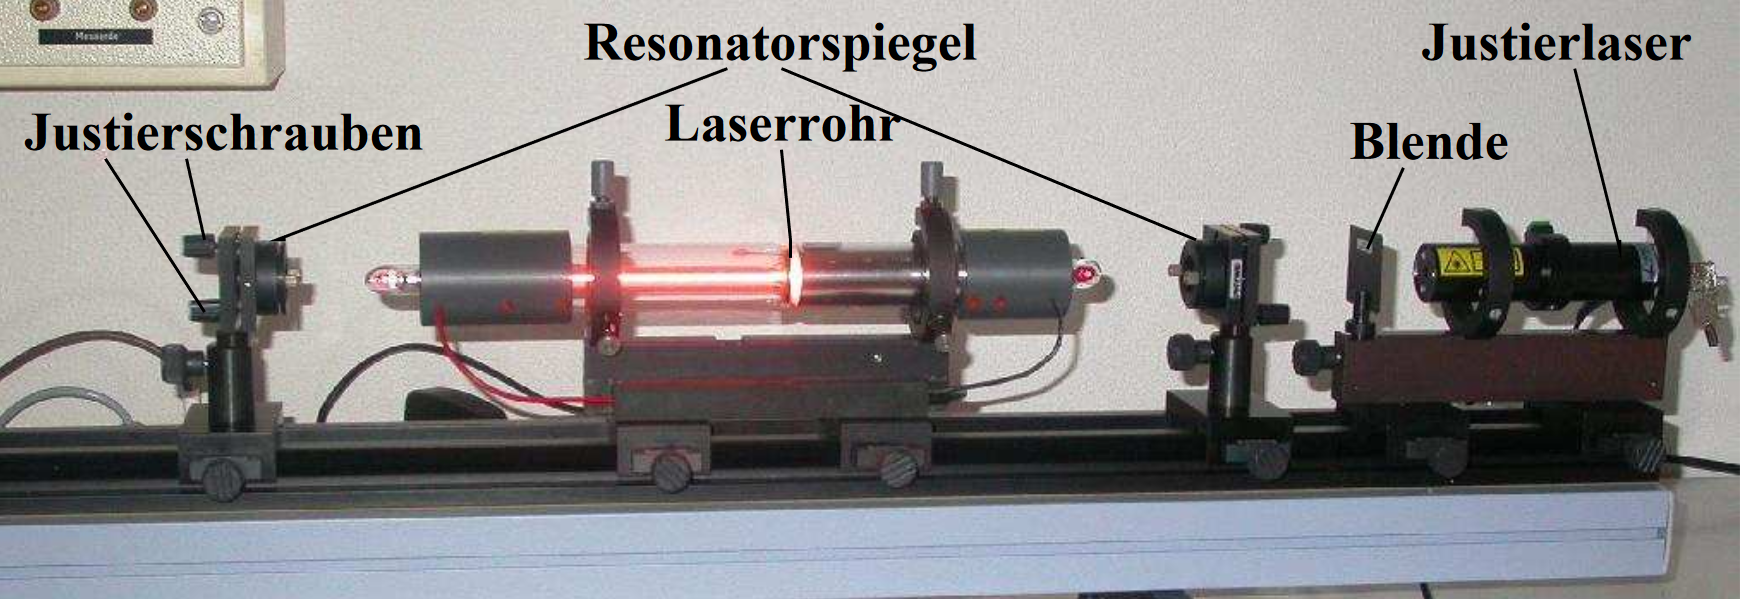
\includegraphics[keepaspectratio,width=0.8\textwidth]{content/images/aufbau.png}
\caption{Versuchsaufbau zur Untersuchung der elementaren Zusammensetzung eines Würfels mittels Tomographie \cite{V14}.}
\label{fig:aufbau}
\end{figure}